\FloatBarrier
\section{ELF format}
\label{sec:elf-format}

Once decided to use this technique for tagging packages, by
using the hash of the package's build script and
dependencies, they key aspect to understand is how this
translates into the underlying file format using by Linux:
ELF. It stands for \textit{Executable and Linkable Format}.
This file format is used both in Linux and the BSD family of
operating systems, and consists of header and symbol tables,
that wrap the underlying assembly to be executed by the
processor \cite{LinuxFoundationReferenced}. The ELF format
is used by any CPU architecture that Linux supports, so the
ELF format is just a ``container'' for the assembly that is
to be executed.

\begin{figure}[hbt]
    \centerfloat
    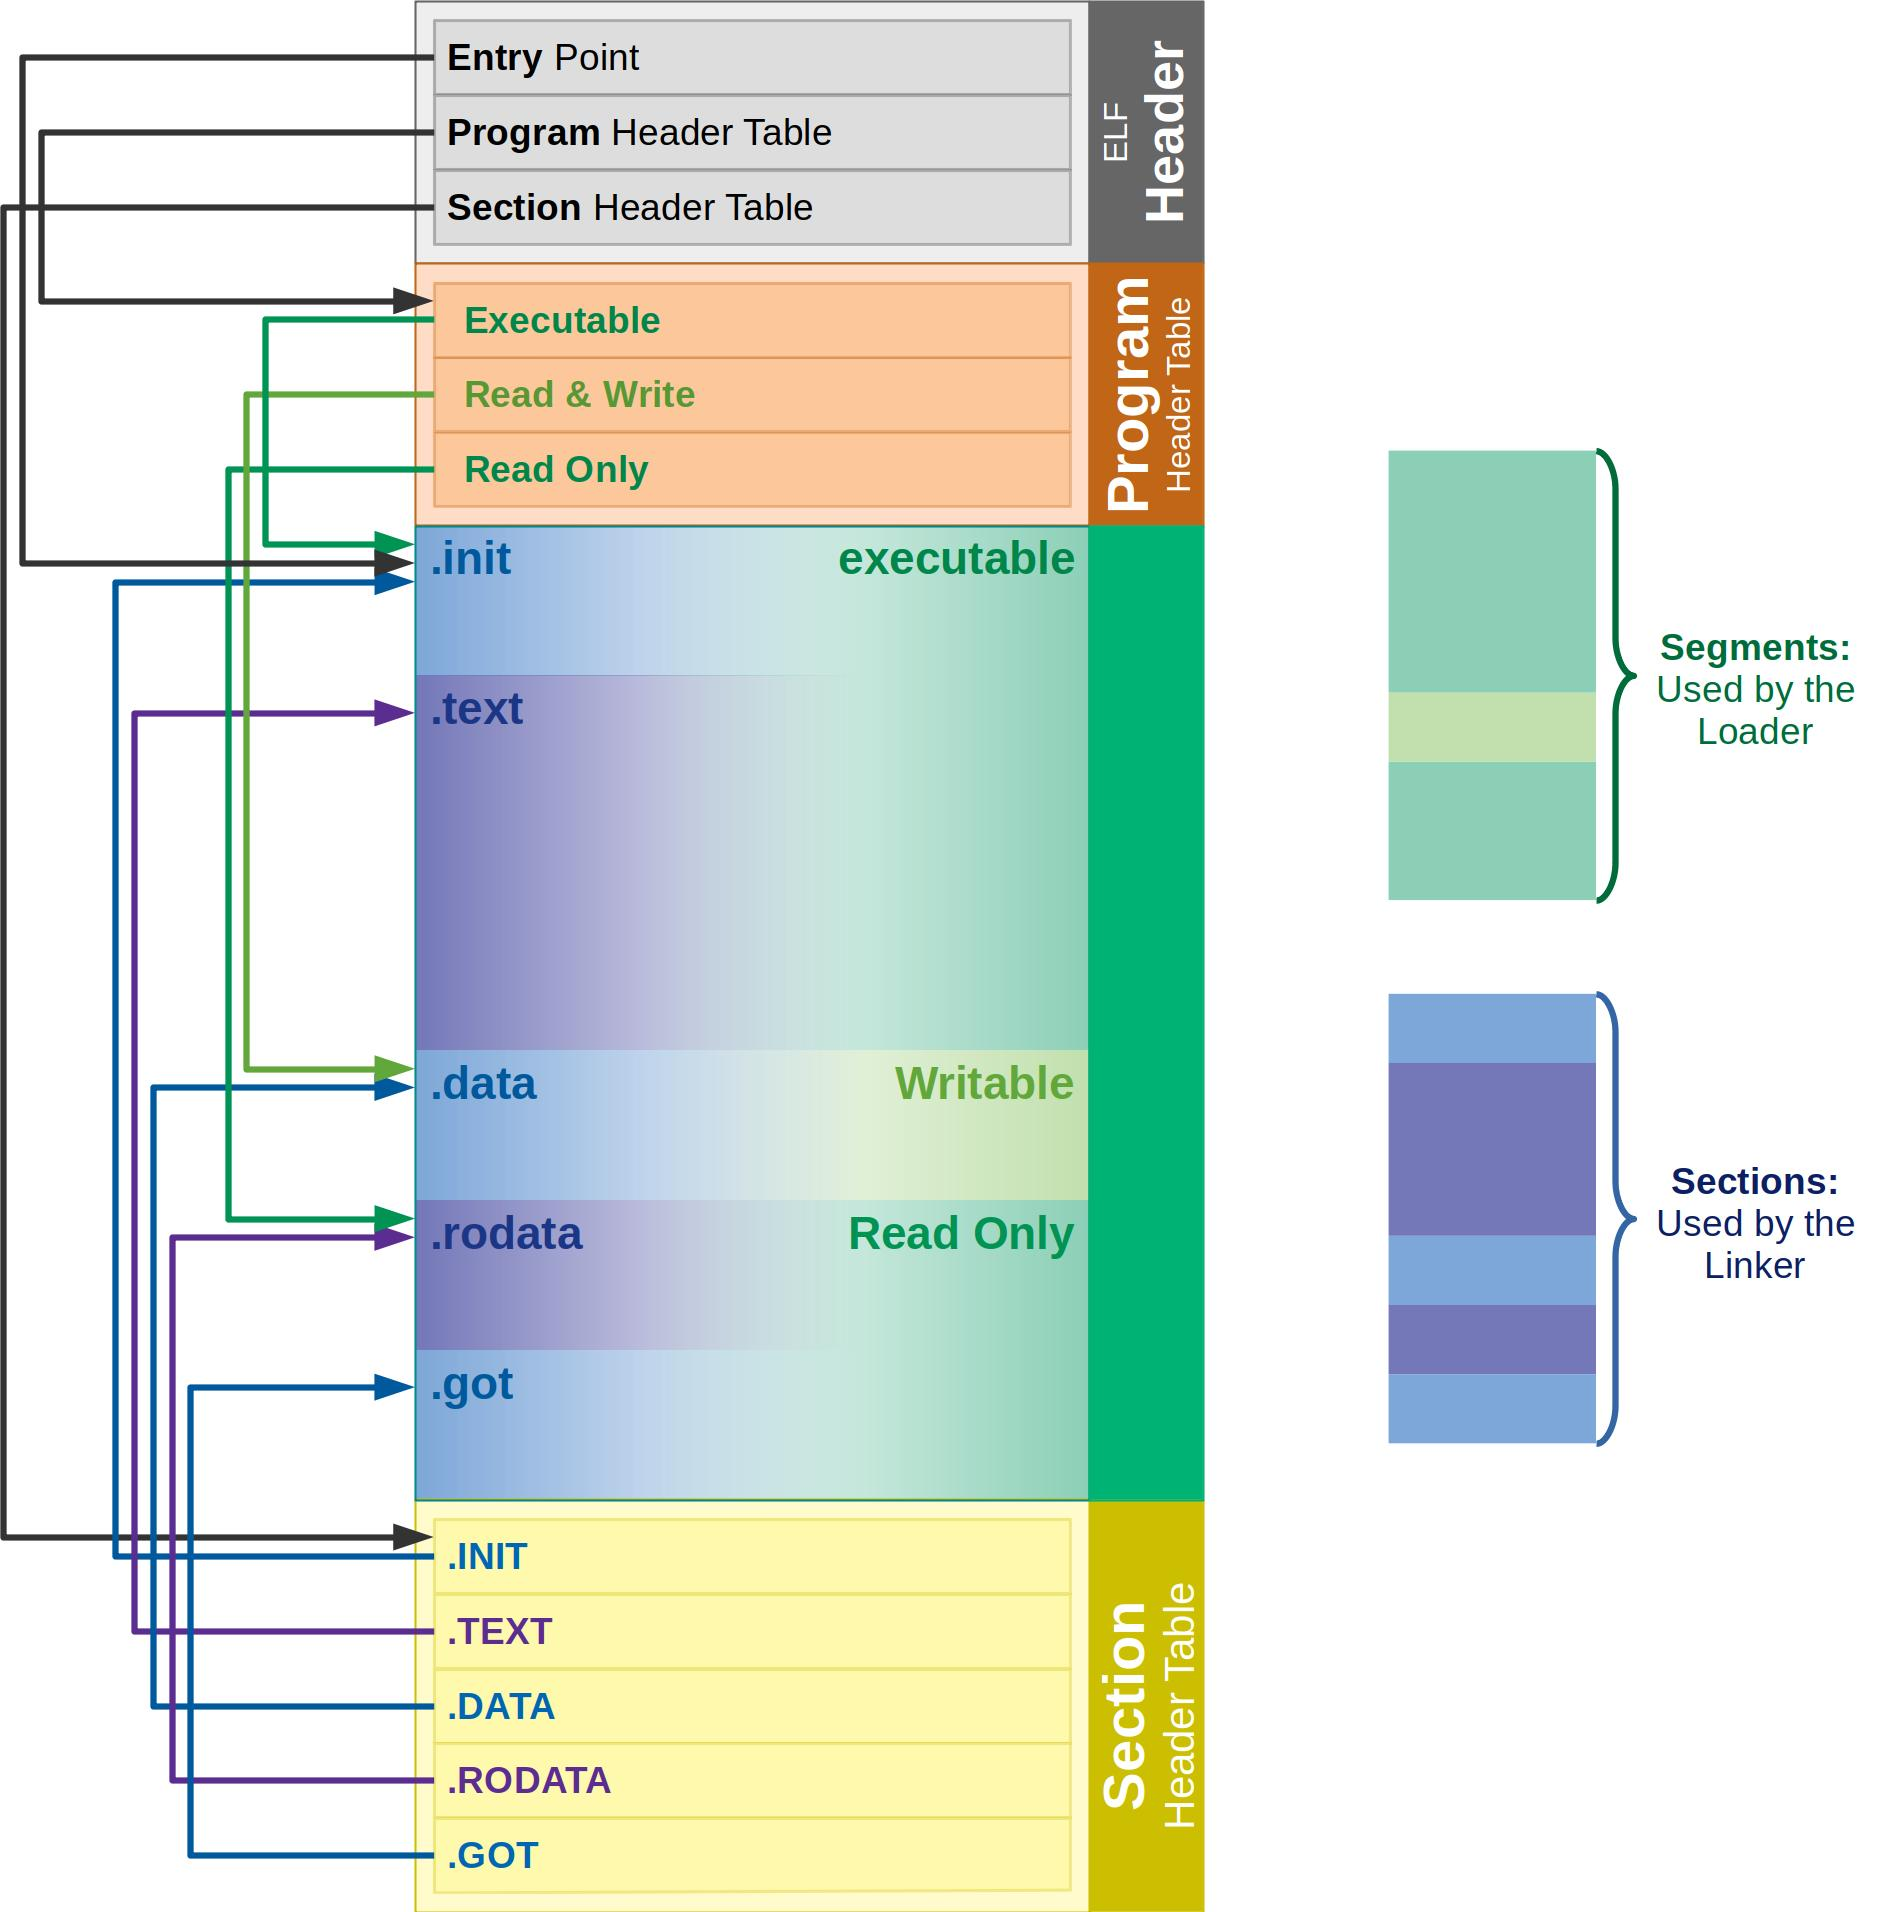
\includegraphics[width=300pt]{assets/typical_elf.jpg}
    \caption{Typical ELF file layout \cite{HW3238POperating}.}
    \label{fig:elf-layout}
\end{figure}


    \begin{minted}{text}
    $ fq .header /usr/bin/ls
        |00 01 02 03 04 05 06 07|01234567|.header{}:
    0x00|7f 45 4c 46 02 01 01 00|.ELF....|  ident{}:
    0x08|00 00 00 00 00 00 00 00|........|
    0x10|03 00                  |..      |  type: "dyn" (0x3)
    0x10|      3e 00            |  >.    |  machine: "x86_64" (0x3e)
    \end{minted}


An ELF file composed of headers, which contains some
metadata about the file itself, segments containing the
actual code and some more metadata at the end. For the scope
of a package manager, it is of interest the study of this
data that is store on an ELF. It is also important to note
that there are two types of executable ELF's:

\begin{itemize}
    \item Statically linked executables
    \item Dynamically linked executables
\end{itemize}

Statically linked executable are usually not distributed by
Linux operating systems. Static executables bundle every
link-time dependency, such that everything is contained in a
single file. So from a distributor's point of view, it
doesn't make sense to make every file bundle every single
dependency, as they could be shared by other components of
the operating system. And some libraries even harder to
statically link, sometimes making it impossible in practice.

Dynamically linked executables and libraries, on the other
hand, rely on parts of the ELF metadata to be able to
discover other dependencies. When an executable is loaded,
via the |exec| system call, the following (non-exhaustive) steps are
performed by the kernel:

\begin{itemize}
    \item The kernel reds the \acl{PHT} which contains
    |INTERP|, this is the requested interpreter for the
    binary.
    \begin{minted}[breaklines]{text}
$ eu-readelf -l /usr/bin/ls
Program Headers:
  INTERP         0x000318 0x0000000000000318 0x0000000000000318 0x00001c 0x00001c R   0x1
        [Requesting program interpreter: /lib64/ld-linux-x86-64.so.2]
  ...
    \end{minted}
    \item Control is transferred to the loader, in this case
    |ld-linux-x86-64.so.2| .
    \item The loader then looks into a different section:
    the |.dynamic|
    \begin{minted}[breaklines]{text}
$ eu-readelf -d /usr/bin/ls
Dynamic segment contains 24 entries:
 Addr: 0x0000000000021a98  Offset: 0x020a98  Link to section: [ 7] '.dynstr'
  Type              Value
  NEEDED            Shared library: [libselinux.so.1]
  NEEDED            Shared library: [libc.so.6]
...
\end{minted}
    \item For each |NEEDED| library, the loader opens it and
    performs the symbol relocations to load them into
    memory.
    \item Finally, the control is transferred into the
    |_start| symbol, which performs some actions and then
    loads the |main| function for a C program.
\end{itemize}

This link loader (also known as dynamic linker) is part of
libc, one of the most important libraries in a Linux
operating system, that provides the standard C library. What
is important from the package manager's perspective, is how
ld-linux loads the dependencies for the |NEEDED| sections.
The manual page for |ld.so| \cite{LdLinuxManual} explains
the following behavior:

\begin{minted}[breaklines]{text}
If a shared object dependency does not contain a slash, then it
is searched for in the following order:

o  Using the directories specified in the DT_RPATH dynamic
   section attribute of the binary if present and DT_RUNPATH
   attribute does not exist.  Use of DT_RPATH is deprecated.

o  Using the environment variable LD_LIBRARY_PATH, unless the
   executable is being run in secure-execution mode (see below),
   in which case this variable is ignored.

o  Using the directories specified in the DT_RUNPATH dynamic
   section attribute of the binary if present.  Such directories
   are searched only to find those objects required by DT_NEEDED
   (direct dependencies) entries and do not apply to those
   objects' children, which must themselves have their own
   DT_RUNPATH entries.  This is unlike DT_RPATH, which is applied
   to searches for all children in the dependency tree.

o  From the cache file /etc/ld.so.cache, which contains a
   compiled list of candidate shared objects previously found in
   the augmented library path.  If, however, the binary was
   linked with the -z nodeflib linker option, shared objects in
   the default paths are skipped.  Shared objects installed in
   hardware capability directories (see below) are preferred to
   other shared objects.

o  In the default path /lib, and then /usr/lib.  (On some 64-bit
   architectures, the default paths for 64-bit shared objects are
   /lib64, and then /usr/lib64.)  If the binary was linked with
   the -z nodeflib linker option, this step is skipped.
\end{minted}

Usually for a conventional Linux distribution, the last
option is the most transversed. That is, loading file from
the default search path in |/usr/lib| or |/lib|. However,
for the software deployment model proposed in the previous
sections, packages don't link again the default search path,
as this causes the issues already explained.
|/etc/ld.so.cache| is also a shorthand for adding
globally-available libraries into the search path.

Finally, what the ELF format provides is the |RUNPATH|
section, which is searched for libraries contained in the
|NEEDED| sections. This |RUNPATH| is very useful, as it
allows every single binary file, to know where to look for
its own hashed dependencies. The link loader can also be
changed to a specific version, instead of relying on a
global |ld-linux.so|. This is done by changing the
|INTERP| in the \ac{PHT}.


As an alternative to a global search path such as the
following layout:

\begin{minted}{text}
INTERP   /lib/ld-linux.so.6
NEEDED   Shared library: [libc.so.6]
RUNPATH  -
\end{minted}

The following layout for an ELF file can be constructed:

\begin{minted}{text}
INTERP   /miq/store/libc-hashAAA/lib/ld-linux.so.6
NEEDED   Shared library: [libc.so.6]
RUNPATH  Library runpath: [/miq/store/libc-hashAAA/lib]
\end{minted}

With a modification of the ELF file metadata, then it is
possible to have a file load exactly the dependencies that
are computed at build time, to support the deployment model
discussed previously. The following chapter describes how
this modification of the ELF metadata is performed.

\FloatBarrier
\section{Other file types}

Not every file in a Linux system is a binary (ELF) file
however. A common Linux system is composed of many ``glue''
shell scripts, or any other text-based file. These files,
also perform the same ``dependency resolving'' that is done
in an ELF, but in a different way. For example, a shell
script that contains the following content:

\begin{minted}{sh}
#!/bin/sh

for file in /srv/backup/*; do
    cp $file /srv/backup2/
    chmod 600 /srv/backup2/$file
done
\end{minted}

A shell script like this also performs another type of
dependency resolution at run-time: loading any existing
program from |PATH|. In this case, both the |cp| and |chmod|
programs are external to the script, and also implicitly
dependencies of itself. For a toy script, it is easy to
underestimate this type of dependency resolution (as |cp|
and |chmod| are included in every Linux distribution), but
as scripts grow bigger, with more and more dependencies, it
becomes hard to keep track of every package.

The first line contains the |#!| sequence, which is called a
``shebang''. Analogous to the ELF format and |ld-linux|, the
shebang instruct Linux to load the program in this path, and
pass the rest of the file into it for execution. In turn
``sh'', interprets the rest of the file as a shell script,
and when faced with the |cp| and |chmod| commands, it reads
the environment variable |PATH|. This is also analogous to
the |RUNPATH| section of a ELF file, but contains
directories with executables:

\begin{minted}[breaklines]{text}
$ printenv PATH | tr ':' '\n'
/usr/local/sbin
/usr/local/bin
/usr/sbin
/usr/bin
/sbin
/bin
/usr/games
/usr/local/games
/usr/lib/wsl/lib
/snap/bin
\end{minted}

These folders are scanned sequentially, until the first
match is found -- that is |/usr/local/sbin/cp|, |/usr/local/bin/cp|, etc.

To avoid this kind of ``implicit'' dependency resolution,
one could also try to use the same technique used for ELF,
namely changing the |RUNPATH|. Unfortunately, this is not
possible, as scripts don't contain any extra ``metadata''
attached to them. A different solution is to construct a
shell script that contains full paths into the required
programs, and their full hashed paths in the store:

\begin{minted}{sh}
#!/miq/store/sh-version-hashAAA/bin/sh

for file in /srv/backup/*; do
    /miq/store/coreutils-version-hashAAA/bin/cp $file /srv/backup2/
    /miq/store/coreutils-version-hashAAA/bin/chmod 600 /srv/backup2/$file
done
\end{minted}

Doing these modifications is not as seamless as tweaking some
compile and link flags for an ELF file, and an automation
tool would be required to resolve the implicit dependencies
of a shell script.

The list of language-specific tweaks would continue -- for
example |PYTHONPATH| for Python packages -- but for the sake
of simplicity, only shell scripts and binary ELF files are
considered in this project. Usually each language ecosystem
has each own method of dependency resolution that can be
overridden to not use a ``global'' search path.
